\documentclass[letterpaper,10pt]{article}
\usepackage{fullpage}
\usepackage{amsmath}
\usepackage{amssymb}
\usepackage{color}
\usepackage{fancyhdr}
\usepackage{multirow}
%\usepackage{graphicx}
\usepackage{tikz}
\pagestyle{fancyplain}
\newcommand\N{\ensuremath{\mathbb N}}
\newcommand\R{\ensuremath{\mathbb R}}
\newcommand\T{\ensuremath{\mathcal T}}
\newcommand\Oh{\ensuremath{\mathcal O}}
\newcommand\Red[1]{\textcolor{red}{\bf #1}}
\newcommand\Blue[1]{\textcolor{blue}{\bf #1}}
\newcommand\Black[1]{\textcolor{black}{#1}}
\begin{document}
%\includegraphics{}

\lhead{CS-471 \\
November 23, 2011}
\rhead{Nick Sorrell \\
Group 11-solo}
\begin{flushleft}
~\\
~\\
%%%%%%%%%%%%%%%%
%	#1	-	%p 166, #4.46
%%%%%%%%%%%%%%%%
\fbox{1} ~~ 
\begin{itemize}
\item[a.]Sketch the trees in $F$.\\
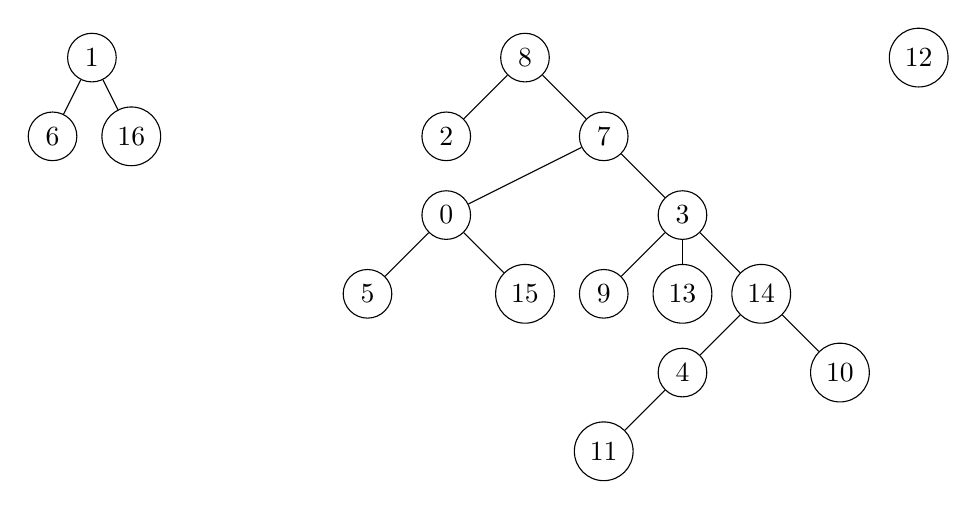
\begin{tikzpicture}
\node (1) at (5,0) [circle, draw] {$1$};
	\node (6) at (4.5,-1) [circle, draw] {$6$} 		edge[-] (1);
	\node (16) at (5.5,-1) [circle, draw] {$16$} 		edge[-] (1);
\node (8) at (10.5,0) [circle, draw] {$8$}; 
	\node (2) at (9.5,-1) [circle, draw] {$2$} 		edge[-] (8);
	\node (7) at (11.5,-1) [circle, draw] {$7$} 		edge[-] (8);
		\node (0) at (9.5,-2) [circle, draw] {$0$} 		edge[-] (7);
			\node (5) at (8.5,-3) [circle, draw] {$5$} 			edge[-] (0);
			\node (15) at (10.5,-3) [circle, draw] {$15$} 		edge[-] (0);	
		\node (3) at (12.5,-2) [circle, draw] {$3$} 		edge[-] (7);
			\node (9) at (11.5,-3) [circle, draw] {$9$} 			edge[-] (3);
			\node (13) at (12.5,-3) [circle, draw] {$13$} 		edge[-] (3);	
			\node (14) at (13.5,-3) [circle, draw] {$14$} 		edge[-] (3);
				\node (4) at (12.5,-4) [circle, draw] {$4$} 			edge[-] (14);
					\node (11) at (11.5,-5) [circle, draw] {$11$} 			edge[-] (4);
				\node (10) at (14.5,-4) [circle, draw] {$10$} 		edge[-] (14);	
\node (12) at (15.5,0) [circle, draw] {$12$};
\end{tikzpicture}


\item[b.] Show the state of $parent[0:16]$ after a call to $Union(Parent[0:16],1,8)$\\
\begin{tikzpicture}
\node (1) at (7,-1) [circle, draw] {$1$}				edge[-](8);
	\node (6) at (6.5,-2) [circle, draw] {$6$} 		edge[-] (1);
	\node (16) at (7.5,-2) [circle, draw] {$16$} 		edge[-] (1);
\node (8) at (10.5,0) [circle, draw] {$8$}; 
	\node (2) at (9.5,-1) [circle, draw] {$2$} 		edge[-] (8);
	\node (7) at (11.5,-1) [circle, draw] {$7$} 		edge[-] (8);
		\node (0) at (9.5,-2) [circle, draw] {$0$} 		edge[-] (7);
			\node (5) at (8.5,-3) [circle, draw] {$5$} 			edge[-] (0);
			\node (15) at (10.5,-3) [circle, draw] {$15$} 		edge[-] (0);	
		\node (3) at (12.5,-2) [circle, draw] {$3$} 		edge[-] (7);
			\node (9) at (11.5,-3) [circle, draw] {$9$} 			edge[-] (3);
			\node (13) at (12.5,-3) [circle, draw] {$13$} 		edge[-] (3);	
			\node (14) at (13.5,-3) [circle, draw] {$14$} 		edge[-] (3);
				\node (4) at (12.5,-4) [circle, draw] {$4$} 			edge[-] (14);
					\node (11) at (11.5,-5) [circle, draw] {$11$} 			edge[-] (4);
				\node (10) at (14.5,-4) [circle, draw] {$10$} 		edge[-] (14);	
\node (12) at (15.5,0) [circle, draw] {$12$};
\end{tikzpicture}

\begin{center}
\begin{tabular}{| r || r | r | r | r | r | r | r | r | r | r | r | r | r | r | r | r | r | r |}
	\hline
	\textbf{$i$} & \textbf{0} & \textbf{1} & \textbf{2} & \textbf{3} & \textbf{4} & \textbf{5} & \textbf{6} & \textbf{7} & \textbf{8} & \textbf{9} & \textbf{10} & 	\textbf{11} & \textbf{12} & \textbf{13} & \textbf{14} & \textbf{15} & \textbf{16} \\
	\hline
	\textbf{$Parent[i]$} & \textbf{7} & \textbf{8} & \textbf{8} & \textbf{7} & \textbf{14} & \textbf{0} & \textbf{1} & \textbf{8} & \textbf{-16} & \textbf{3} & \textbf{14} & \textbf{4} & \textbf{-1} & \textbf{3} & \textbf{3} & \textbf{0} & \textbf{1} \\
	\hline
\end{tabular}
\end{center}

\newpage
\item[c.] Given the state of $Parent[0:16]$ in part (b), show the state of  $Parent[0:16]$ after an invocation of $Find(Parent[0:16],4)$ and sketch the trees in $F$.\\
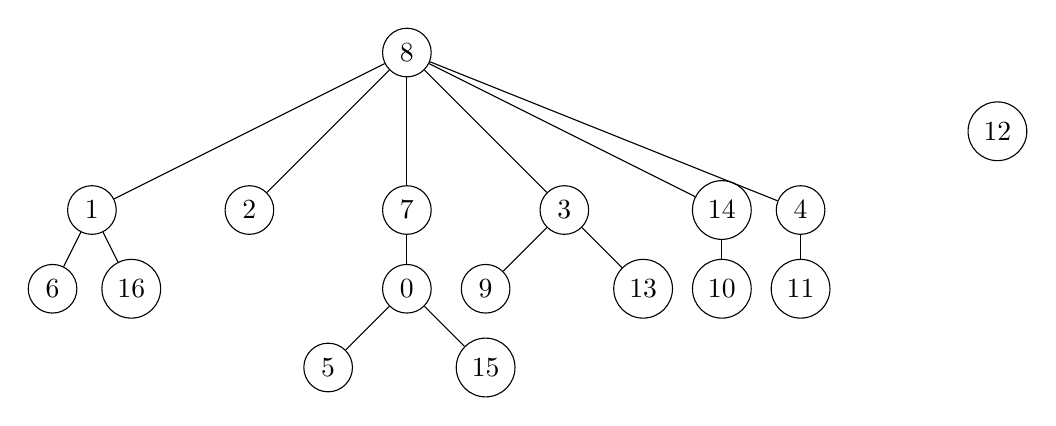
\begin{tikzpicture}
\node (8) at (11,1) [circle, draw] {$8$}; 
	\node (1) at (7,-1) [circle, draw] {$1$}				edge[-](8);
		\node (6) at (6.5,-2) [circle, draw] {$6$} 		edge[-] (1);
		\node (16) at (7.5,-2) [circle, draw] {$16$} 		edge[-] (1);
	\node (2) at (9,-1) [circle, draw] {$2$} 		edge[-] (8);
	\node (7) at (11,-1) [circle, draw] {$7$} 		edge[-] (8);
		\node (0) at (11,-2) [circle, draw] {$0$} 		edge[-] (7);
			\node (5) at (10,-3) [circle, draw] {$5$} 		edge[-] (0);
			\node (15) at (12,-3) [circle, draw] {$15$} 		edge[-] (0);	
	\node (3) at (13,-1) [circle, draw] {$3$} 		edge[-] (8);
		\node (9) at (12,-2) [circle, draw] {$9$} 			edge[-] (3);
		\node (13) at (14,-2) [circle, draw] {$13$} 		edge[-] (3);	
	\node (14) at (15,-1) [circle, draw] {$14$} 		edge[-] (8);
		\node (10) at (15,-2) [circle, draw] {$10$} 		edge[-] (14);	
	\node (4) at (16,-1) [circle, draw] {$4$} 		edge[-] (8);
		\node (11) at (16,-2) [circle, draw] {$11$} 		edge[-] (4);
\node (12) at (18.5,0) [circle, draw] {$12$};
\end{tikzpicture}

\begin{center}
\begin{tabular}{| r || r | r | r | r | r | r | r | r | r | r | r | r | r | r | r | r | r | r |}
	\hline
	\textbf{$i$} & \textbf{0} & \textbf{1} & \textbf{2} & \textbf{3} & \textbf{4} & \textbf{5} & \textbf{6} & \textbf{7} & \textbf{8} & \textbf{9} & \textbf{10} & 		\textbf{11} & \textbf{12} & \textbf{13} & \textbf{14} & \textbf{15} & \textbf{16} \\
	\hline
	\textbf{$Parent[i]$} & \textbf{7} & \textbf{8} & \textbf{8} & \textbf{7} & \textbf{14} & \textbf{0} & \textbf{1} & \textbf{8} & \textbf{-16} & \textbf{3} & \textbf{14} & \textbf{4} & \textbf{-1} & \textbf{3} & \textbf{3} & \textbf{0} & \textbf{1} \\
	\hline
\end{tabular}
\end{center}

\end{itemize}
~\\

%%%%%%%%%%%%%%%%
%	#2	-	p 161, #4.13
%%%%%%%%%%%%%%%%
\fbox{2} State and prove a generalization for $k$-ary trees: 
~\\
 \begin{itemize}
\item[a.]Given that the depth of a complete binary tree $T_n$ is given by\\
$d(T_n)=\lfloor$log$_2n \rfloor$. \\
~\\
If $T$ is a complete $k$-ary tree, then the number of nodes, $n$, we have \\ 
\begin{eqnarray*}
n &\leq& 1 + k + \cdots + k^d\\
&=& \frac{k^{d+1}-1}{k-1}\\
n(k-1) &\leq& k^{d+1}\\
\text{log}_k(n(k-1)) &\leq& d+1 \\
\text{log}_k(n(k-1))-1 &\leq& d \\
\end{eqnarray*}

And since $d$, the depth of the tree, is an integer, we can take the ceiling of that expression as our answer.

\item[c.] For any $k-tree$, we will have $k$ leaves for each internal node.  Thus, proposition 4.2.3 states for 2-trees that\\
$I(T)=L(T)-1$\\
This could be equivalently written for a 2-tree, where $k=2$\\
$I(T)=\frac{L(T)-1}{k-1}=\frac{L(T)-1}{1}$ \\
That holds for the base case, and\\
$I(T)=\frac{L(T)-1}{k-1}$ \\
holds in the general case of $k-trees$
\end{itemize}

\newpage
%%%%%%%%%%%%%%%%
%	#3	-	P 391, #12.1
%%%%%%%%%%%%%%%% 
 \fbox{3} ~~
 \begin{itemize}
\item[a.] Trace the action of procedure $Kruskal$ for $G$. \\
Implemented with Graph ADT, Priority Queue ADT, Forest ADT using Parent array, Collection of Disjoint Node sets. \\
~\\

\begin{tabular}{| r || r | r | r | r | r | r | r | r |}
	\multicolumn{9}{l}{Step 0: Initial Conditions}\\
	\hline
	\textbf{$i$} & \textbf{0} & \textbf{1} & \textbf{2} & \textbf{3} & \textbf{4} & \textbf{5} & \textbf{6} & \textbf{7} \\
	\hline
	\textbf{$Parent[i]$} & \textbf{-1} & \textbf{-1} & \textbf{-1} & \textbf{-1} & \textbf{-1} & \textbf{-1} & \textbf{-1} & \textbf{-1} \\
	\hline
	\textbf{Node sets} & \multicolumn{7}{l}{\{0\},\{1\},\{2\},\{3\},\{4\},\{5\},\{6\},\{7\}} & \\
	\hline
	\textbf{Selected edge} & \multicolumn{7}{l}{\{\}} & \\
	\hline
\end{tabular}
~\\
\begin{tabular}{| r | r | r | r | r | r | r | r | r | r | r |}
	\multicolumn{10}{l}{Step 1: Select edge 5-6 between Nodes }\\
	\hline
	\multirow{4}{*}{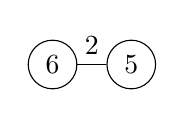
\begin{tikzpicture}
		\node (6) at (1,0) [circle, draw] {$6$}; 
			\node (5) at (2,0) [circle, draw] {$5$}				edge[-](6);
		\draw (5) to node [above] {2} (6);
		\end{tikzpicture}}
	&~& \textbf{$i$} & 				\textbf{0} & \textbf{1} & \textbf{2} & \textbf{3} & \textbf{4} & \textbf{5} & \textbf{6} & \textbf{7} \\
	&~& \textbf{$Parent[i]$} & 		\textbf{-1} & \textbf{-1} & \textbf{-1} & \textbf{-1} & \textbf{-1} & \textbf{-2} & \textbf{5} & \textbf{-1} \\
	&~& \textbf{Node sets} & \multicolumn{7}{l}{\{0\},\{1\},\{2\},\{3\},\{4\},\{5,6\},\{7\}} & \\
	&~& \textbf{Selected edge} & \multicolumn{7}{l}{\{5-6\}} & \\
		&~& ~& \multicolumn{7}{l}{~} & \\
	\hline
\end{tabular}

\begin{tabular}{| r | r | r | r | r | r | r | r | r | r | r |}
	\multicolumn{10}{l}{Step 2: Select edge 0-5 between Nodes }\\
	\hline
	\multirow{4}{*}{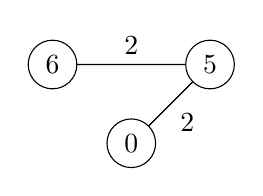
\begin{tikzpicture}
	\node (6) at (1,0) [circle, draw] {$6$}; 
		\node (5) at (3,0) [circle, draw] {$5$}				edge[-](6);
			\node (0) at (2,-1) [circle, draw] {$0$}		edge[-](5);
	\draw (5) to node [above] {2} (6)
		  (0) to node [below right] {2} (5);
	\end{tikzpicture}}
	&~& \textbf{$i$} & 			\textbf{0} & \textbf{1} & \textbf{2} & \textbf{3} & \textbf{4} & \textbf{5} & \textbf{6} & \textbf{7} \\
	&~& \textbf{$Parent[i]$} &  \textbf{5} & \textbf{-1} & \textbf{-1} & \textbf{-1} & \textbf{-1} & \textbf{-3} & \textbf{5} & \textbf{-1} \\
	&~& \textbf{Node sets} & \multicolumn{7}{l}{\{1\},\{2\},\{3\},\{4\},\{0,5,6\},\{7\}} & \\
	&~& \textbf{Selected edge} & \multicolumn{7}{l}{\{0-5\}} & \\
	&~& ~& \multicolumn{7}{l}{~} & \\
	\hline
\end{tabular}

\begin{tabular}{| r | r | r | r | r | r | r | r | r | r | r |}
	\multicolumn{10}{l}{Step 3: Select edge 4-3 between Nodes }\\
	\hline
	\multirow{4}{*}{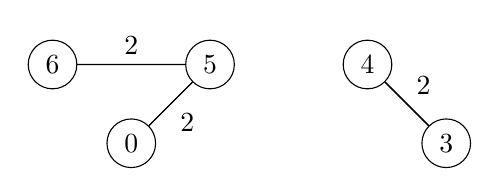
\begin{tikzpicture}
	\node (6) at (1,0) [circle, draw] {$6$}; 
		\node (5) at (3,0) [circle, draw] {$5$}				edge[-](6);
			\node (0) at (2,-1) [circle, draw] {$0$}		edge[-](5);
	\node (4) at (5,0) [circle, draw] {$4$};
		\node (3) at (6,-1) [circle, draw] {$3$}				edge[-](4);
	\draw (5) to node [above] {2} (6)
		  (0) to node [below right] {2} (5)
		  (3) to node [above right] {2} (4);
	\end{tikzpicture}}
	&~& \textbf{$i$} & 			\textbf{0} & \textbf{1} & \textbf{2} & \textbf{3} & \textbf{4} & \textbf{5} & \textbf{6} & \textbf{7} \\
	&~& \textbf{$Parent[i]$} &	\textbf{5} & \textbf{-1} & \textbf{-1} & \textbf{4} & \textbf{-2} & \textbf{-3} & \textbf{5} & \textbf{-1} \\
	&~& \textbf{Node sets} & \multicolumn{7}{l}{\{1\},\{2\},\{3,4\},\{0,5,6\},\{7\}} & \\
	&~& \textbf{Selected edge} & \multicolumn{7}{l}{\{4-3\}} & \\
	&~& ~& \multicolumn{7}{l}{~} & \\
	\hline
\end{tabular}

\begin{tabular}{| r | r | r | r | r | r | r | r | r | r | r |}
	\multicolumn{10}{l}{Step 4: Select edge 5-1 between Nodes }\\
	\hline
	\multirow{4}{*}{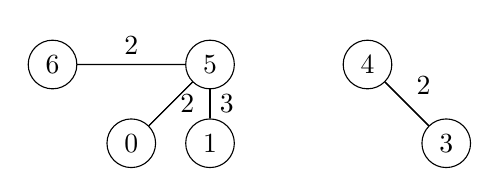
\begin{tikzpicture}
	\node (6) at (1,0) [circle, draw] {$6$}; 
		\node (5) at (3,0) [circle, draw] {$5$}				edge[-](6);
			\node (0) at (2,-1) [circle, draw] {$0$}		edge[-](5);
			\node (1) at (3, -1) [circle, draw] {$1$}		edge[-](5);
	\node (4) at (5,0) [circle, draw] {$4$};
		\node (3) at (6,-1) [circle, draw] {$3$}				edge[-](4);
	\draw (5) to node [above] {2} (6)
		  (0) to node [right] {2} (5)
		  (3) to node [above right] {2} (4)
		  (1) to node [right] {3} (5);
	\end{tikzpicture}}
	&~& \textbf{$i$} & 			\textbf{0} & \textbf{1} & \textbf{2} & \textbf{3} & \textbf{4} & \textbf{5} & \textbf{6} & \textbf{7} \\
	&~& \textbf{$Parent[i]$} &	\textbf{5} & \textbf{5} & \textbf{-1} & \textbf{4} & \textbf{-2} & \textbf{-4} & \textbf{5} & \textbf{-1} \\
	&~& \textbf{Node sets} & \multicolumn{7}{l}{\{2\},\{3,4\},\{0,1,5,6\},\{7\}} & \\
	&~& \textbf{Selected edge} & \multicolumn{7}{l}{\{5-1\}} & \\
	&~& ~& \multicolumn{7}{l}{~} & \\
	\hline
\end{tabular}

\begin{tabular}{| r | r | r | r | r | r | r | r | r | r | r |}
	\multicolumn{10}{l}{Step 5: Select edge 4-2 between Nodes }\\
	\hline
	\multirow{4}{*}{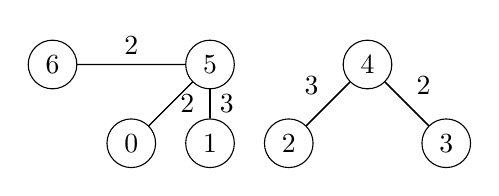
\begin{tikzpicture}
	\node (6) at (1,0) [circle, draw] {$6$}; 
		\node (5) at (3,0) [circle, draw] {$5$}				edge[-](6);
			\node (0) at (2,-1) [circle, draw] {$0$}		edge[-](5);
			\node (1) at (3, -1) [circle, draw] {$1$}		edge[-](5);
	\node (4) at (5,0) [circle, draw] {$4$};
		\node (3) at (6,-1) [circle, draw] {$3$}				edge[-](4);
		\node (2) at (4,-1) [circle, draw] {$2$}			edge[-](4);
	\draw (5) to node [above] {2} (6)
		  (0) to node [right] {2} (5)
		  (3) to node [above right] {2} (4)
		  (1) to node [right] {3} (5)
		  (2) to node [above left] {3} (4);
	\end{tikzpicture}}
	&~& \textbf{$i$} & 			\textbf{0} & \textbf{1} & \textbf{2} & \textbf{3} & \textbf{4} & \textbf{5} & \textbf{6} & \textbf{7} \\
	&~& \textbf{$Parent[i]$} &	\textbf{5} & \textbf{5} & \textbf{4} & \textbf{4} & \textbf{-3} & \textbf{-4} & \textbf{5} & \textbf{-1} \\
	&~& \textbf{Node sets} & \multicolumn{7}{l}{\{2,3,4\},\{0,1,5,6\},\{7\}} & \\
	&~& \textbf{Selected edge} & \multicolumn{7}{l}{\{4-2\}} & \\
	&~& ~& \multicolumn{7}{l}{~} & \\
	\hline
\end{tabular}

\begin{tabular}{| r | r | r | r | r | r | r | r | r | r | r |}
	\multicolumn{10}{l}{Step 6: Select edge 0-7 between Nodes }\\
	\hline
	\multirow{4}{*}{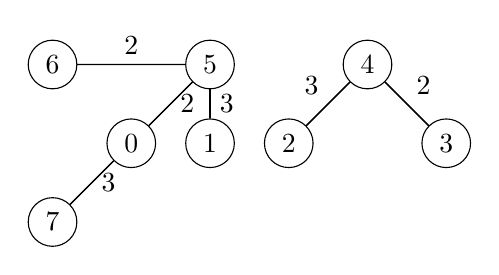
\begin{tikzpicture}
	\node (6) at (1,0) [circle, draw] {$6$}; 
		\node (5) at (3,0) [circle, draw] {$5$}				edge[-](6);
			\node (0) at (2,-1) [circle, draw] {$0$}		edge[-](5);
				\node (7) at (1,-2) [circle, draw] {$7$}	edge[-](0);
			\node (1) at (3, -1) [circle, draw] {$1$}		edge[-](5);
	\node (4) at (5,0) [circle, draw] {$4$};
		\node (3) at (6,-1) [circle, draw] {$3$}				edge[-](4);
		\node (2) at (4,-1) [circle, draw] {$2$}			edge[-](4);
	\draw (5) to node [above] {2} (6)
		  (0) to node [right] {2} (5)
		  (3) to node [above right] {2} (4)
		  (1) to node [right] {3} (5)
		  (2) to node [above left] {3} (4)
		  (7) to node [right] {3} (0);
	\end{tikzpicture}}
	&~& \textbf{$i$} & 			\textbf{0} & \textbf{1} & \textbf{2} & \textbf{3} & \textbf{4} & \textbf{5} & \textbf{6} & \textbf{7} \\
	&~& \textbf{$Parent[i]$} &	\textbf{5} & \textbf{5} & \textbf{4} & \textbf{4} & \textbf{-3} & \textbf{-4} & \textbf{5} & \textbf{0} \\
	&~& \textbf{Node sets} & \multicolumn{7}{l}{\{2,3,4\},\{0,1,5,6,7\}} & \\
	&~& \textbf{Selected edge} & \multicolumn{7}{l}{\{0-7\}} & \\
	&~& ~& \multicolumn{7}{l}{~} & \\
	&~& ~& \multicolumn{7}{l}{~} & \\
	&~& ~& \multicolumn{7}{l}{~} & \\
	\hline
\end{tabular}

\begin{tabular}{| r | r | r | r | r | r | r | r | r | r | r |}
	\multicolumn{10}{l}{Step 7: Select edge 5-4 between Nodes }\\
	\hline
	\multirow{4}{*}{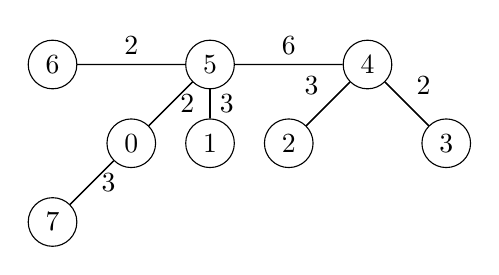
\begin{tikzpicture}
	\node (6) at (1,0) [circle, draw] {$6$}; 
		\node (5) at (3,0) [circle, draw] {$5$}				edge[-](6);
			\node (0) at (2,-1) [circle, draw] {$0$}		edge[-](5);
				\node (7) at (1,-2) [circle, draw] {$7$}	edge[-](0);
			\node (1) at (3, -1) [circle, draw] {$1$}		edge[-](5);
	\node (4) at (5,0) [circle, draw] {$4$};
		\node (3) at (6,-1) [circle, draw] {$3$}				edge[-](4);
		\node (2) at (4,-1) [circle, draw] {$2$}			edge[-](4);
	\draw (5) to node [above] {2} (6)
		  (0) to node [right] {2} (5)
		  (3) to node [above right] {2} (4)
		  (1) to node [right] {3} (5)
		  (2) to node [above left] {3} (4)
		  (7) to node [right] {3} (0)
		  (5) to node [above] {6} (4);
	\end{tikzpicture}}
	&~& \textbf{$i$} & 			\textbf{0} & \textbf{1} & \textbf{2} & \textbf{3} & \textbf{4} & \textbf{5} & \textbf{6} & \textbf{7} \\
	&~& \textbf{$Parent[i]$} &	\textbf{5} & \textbf{5} & \textbf{4} & \textbf{4} & \textbf{5} & \textbf{-5} & \textbf{5} & \textbf{0} \\
	&~& \textbf{Node sets} & \multicolumn{7}{l}{\{0,1,2,3,4,5,6,7\}} & \\
	&~& \textbf{Selected edge} & \multicolumn{7}{l}{\{5-4\}} & \\
	&~& ~& \multicolumn{7}{l}{~} & \\
	&~& ~& \multicolumn{7}{l}{~} & \\
	&~& ~& \multicolumn{7}{l}{~} & \\
	\hline
\end{tabular}


\item[b.] Prim's\\
\begin{tabular}{| r | r | r | r | r | r | r | r | r | r | r |}
	\multicolumn{10}{l}{Stage 1}\\
	\hline
	\multirow{4}{*}{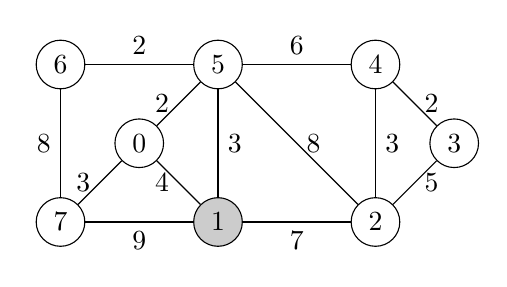
\begin{tikzpicture}
	\node (6) at (-1, 0) [circle, draw] {$6$};
	\node (5) at (1,0) [circle, draw] {$5$};
	\node (4) at (3,0) [circle, draw] {$4$};
		\node (0) at (0,-1) [circle, draw] {$0$};
		\node (3) at (4,-1) [circle, draw] {$3$};
			\node[fill=black!20] (1) at (1, -2) [circle, draw] {$1$};
			\node (7) at (-1, -2) [circle, draw] {$7$};
			\node (2) at (3, -2) [circle, draw] {$2$};
	\draw[-] (0) to node [left] {2} (5);
	\draw[-] (0) to node [left] {3} (7);
	\draw[-] (0) to node [left] {4} (1);
	\draw[-] (1) to node [right] {3} (5);
	\draw[-] (1) to node [below] {7} (2);
	\draw[-] (1) to node [below] {9} (7);
	\draw[-] (2) to node [right] {8} (5);
	\draw[-] (2) to node [right] {3} (4);
	\draw[-] (2) to node [right] {5} (3);
	\draw[-] (3) to node [right] {2} (4);
	\draw[-] (4) to node [above] {6} (5);
	\draw[-] (5) to node [above] {2} (6);
	\draw[-] (6) to node [left] {8} (7);			
	\end{tikzpicture}}
	&~& \textbf{$i$} & 				\textbf{0} & \textbf{1} & \textbf{2} & \textbf{3} & 		\textbf{4} & 		\textbf{5} & \textbf{6} & 		\textbf{7}\\
	&~& \textbf{$Nearest[i]$} & 	\textbf{4} & \textbf{0} & \textbf{7} & \textbf{$\infty$} &  \textbf{$\infty$} & \textbf{3} & \textbf{$\infty$} & \textbf{9}\\
	&~& \textbf{$Parent[i]$} & 		\textbf{1} & \textbf{-1} &\textbf{1} & \textbf{-} & 		\textbf{-} & 		\textbf{1} & \textbf{-} & 		\textbf{1}\\
	&~& \textbf{$InTheTree[i]$} & 	\textbf{F} & \textbf{T} & \textbf{F} & \textbf{F} &		    \textbf{F} & 		\textbf{F} & \textbf{F} & 		\textbf{F}\\
	&~& \textbf{$Weight$}& \multicolumn{7}{l}{0} & \\
	&~& ~& \multicolumn{7}{l}{~} & \\
	&~& ~& \multicolumn{7}{l}{~} & \\
	&~& ~& \multicolumn{7}{l}{~} & \\
	\hline
\end{tabular}

\begin{tabular}{| r | r | r | r | r | r | r | r | r | r | r |}
	\multicolumn{10}{l}{Stage 2}\\
	\hline
	\multirow{4}{*}{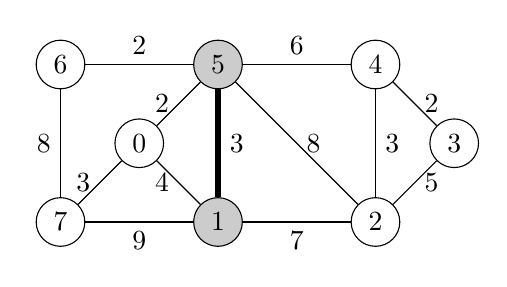
\begin{tikzpicture}
	\node (6) at (-1, 0) [circle, draw] {$6$};
	\node[fill=black!20] (5) at (1,0) [circle, draw] {$5$};
	\node (4) at (3,0) [circle, draw] {$4$};
		\node (0) at (0,-1) [circle, draw] {$0$};
		\node (3) at (4,-1) [circle, draw] {$3$};
			\node[fill=black!20] (1) at (1, -2) [circle, draw] {$1$};
			\node (7) at (-1, -2) [circle, draw] {$7$};
			\node (2) at (3, -2) [circle, draw] {$2$};
	\draw[-] (0) to node [left] {2} (5);
	\draw[-] (0) to node [left] {3} (7);
	\draw[-] (0) to node [left] {4} (1);
	\draw[line width=2pt][-] (1) to node [right] {3} (5);
	\draw[-] (1) to node [below] {7} (2);
	\draw[-] (1) to node [below] {9} (7);
	\draw[-] (2) to node [right] {8} (5);
	\draw[-] (2) to node [right] {3} (4);
	\draw[-] (2) to node [right] {5} (3);
	\draw[-] (3) to node [right] {2} (4);
	\draw[-] (4) to node [above] {6} (5);
	\draw[-] (5) to node [above] {2} (6);
	\draw[-] (6) to node [left] {8} (7);			
	\end{tikzpicture}}
	&~& \textbf{$i$} & 				\textbf{0} & \textbf{1} & \textbf{2} & \textbf{3} & 		\textbf{4} & 		\textbf{5} & \textbf{6} & 		\textbf{7}\\
	&~& \textbf{$Nearest[i]$} & 	\textbf{2} & \textbf{0} & \textbf{7} & \textbf{$\infty$} &  \textbf{6} & 		\textbf{3} & \textbf{2} &		\textbf{9}\\
	&~& \textbf{$Parent[i]$} & 		\textbf{5} & \textbf{-1} &\textbf{1} & \textbf{-} & 		\textbf{5} & 		\textbf{1} & \textbf{5} & 		\textbf{1}\\
	&~& \textbf{$InTheTree[i]$} & 	\textbf{F} & \textbf{T} & \textbf{F} & \textbf{F} &		    \textbf{F} & 		\textbf{T} & \textbf{F} & 		\textbf{F}\\
	&~& \textbf{$Weight$}& \multicolumn{7}{l}{3} & \\
	&~& ~& \multicolumn{7}{l}{~} & \\
	&~& ~& \multicolumn{7}{l}{~} & \\
	&~& ~& \multicolumn{7}{l}{~} & \\
	\hline
\end{tabular}

\begin{tabular}{| r | r | r | r | r | r | r | r | r | r | r |}
	\multicolumn{10}{l}{Stage 3}\\
	\hline
	\multirow{4}{*}{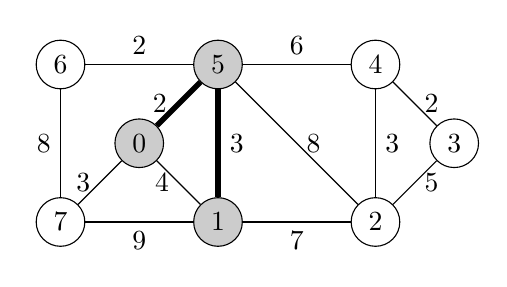
\begin{tikzpicture}
	\node (6) at (-1, 0) [circle, draw] {$6$};
	\node[fill=black!20] (5) at (1,0) [circle, draw] {$5$};
	\node (4) at (3,0) [circle, draw] {$4$};
		\node[fill=black!20] (0) at (0,-1) [circle, draw] {$0$};
		\node (3) at (4,-1) [circle, draw] {$3$};
			\node[fill=black!20] (1) at (1, -2) [circle, draw] {$1$};
			\node (7) at (-1, -2) [circle, draw] {$7$};
			\node (2) at (3, -2) [circle, draw] {$2$};
	\draw[line width=2pt][-] (0) to node [left] {2} (5);
	\draw[-] (0) to node [left] {3} (7);
	\draw[-] (0) to node [left] {4} (1);
	\draw[line width=2pt][-] (1) to node [right] {3} (5);
	\draw[-] (1) to node [below] {7} (2);
	\draw[-] (1) to node [below] {9} (7);
	\draw[-] (2) to node [right] {8} (5);
	\draw[-] (2) to node [right] {3} (4);
	\draw[-] (2) to node [right] {5} (3);
	\draw[-] (3) to node [right] {2} (4);
	\draw[-] (4) to node [above] {6} (5);
	\draw[-] (5) to node [above] {2} (6);
	\draw[-] (6) to node [left] {8} (7);			
	\end{tikzpicture}}
	&~& \textbf{$i$} & 				\textbf{0} & \textbf{1} & \textbf{2} & \textbf{3} & 		\textbf{4} & 		\textbf{5} & \textbf{6} & 		\textbf{7}\\
	&~& \textbf{$Nearest[i]$} & 	\textbf{2} & \textbf{0} & \textbf{7} & \textbf{$\infty$} &  \textbf{6} & 		\textbf{3} & \textbf{2} &		\textbf{3}\\
	&~& \textbf{$Parent[i]$} & 		\textbf{5} & \textbf{-1} &\textbf{1} & \textbf{-} & 		\textbf{5} & 		\textbf{1} & \textbf{5} & 		\textbf{0}\\
	&~& \textbf{$InTheTree[i]$} & 	\textbf{T} & \textbf{T} & \textbf{F} & \textbf{F} &		    \textbf{F} & 		\textbf{T} & \textbf{F} & 		\textbf{F}\\
	&~& \textbf{$Weight$}& \multicolumn{7}{l}{5} & \\
	&~& ~& \multicolumn{7}{l}{~} & \\
	&~& ~& \multicolumn{7}{l}{~} & \\
	&~& ~& \multicolumn{7}{l}{~} & \\
	\hline
\end{tabular}

\begin{tabular}{| r | r | r | r | r | r | r | r | r | r | r |}
	\multicolumn{10}{l}{Stage 4}\\
	\hline
	\multirow{4}{*}{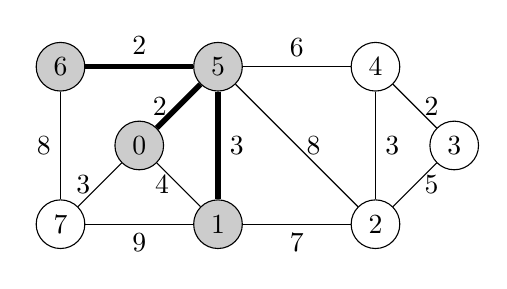
\begin{tikzpicture}
	\node[fill=black!20] (6) at (-1, 0) [circle, draw] {$6$};
	\node[fill=black!20] (5) at (1,0) [circle, draw] {$5$};
	\node (4) at (3,0) [circle, draw] {$4$};
		\node[fill=black!20] (0) at (0,-1) [circle, draw] {$0$};
		\node (3) at (4,-1) [circle, draw] {$3$};
			\node[fill=black!20] (1) at (1, -2) [circle, draw] {$1$};
			\node (7) at (-1, -2) [circle, draw] {$7$};
			\node (2) at (3, -2) [circle, draw] {$2$};
	\draw[line width=2pt][-] (0) to node [left] {2} (5);
	\draw[-] (0) to node [left] {3} (7);
	\draw[-] (0) to node [left] {4} (1);
	\draw[line width=2pt][-] (1) to node [right] {3} (5);
	\draw[-] (1) to node [below] {7} (2);
	\draw[-] (1) to node [below] {9} (7);
	\draw[-] (2) to node [right] {8} (5);
	\draw[-] (2) to node [right] {3} (4);
	\draw[-] (2) to node [right] {5} (3);
	\draw[-] (3) to node [right] {2} (4);
	\draw[-] (4) to node [above] {6} (5);
	\draw[line width=2pt][-] (5) to node [above] {2} (6);
	\draw[-] (6) to node [left] {8} (7);			
	\end{tikzpicture}}
	&~& \textbf{$i$} & 				\textbf{0} & \textbf{1} & \textbf{2} & \textbf{3} & 		\textbf{4} & 		\textbf{5} & \textbf{6} & 		\textbf{7}\\
	&~& \textbf{$Nearest[i]$} & 	\textbf{2} & \textbf{0} & \textbf{7} & \textbf{$\infty$} &  \textbf{6} & 		\textbf{3} & \textbf{2} &		\textbf{3}\\
	&~& \textbf{$Parent[i]$} & 		\textbf{5} & \textbf{-1} &\textbf{1} & \textbf{-} & 		\textbf{5} & 		\textbf{1} & \textbf{5} & 		\textbf{0}\\
	&~& \textbf{$InTheTree[i]$} & 	\textbf{T} & \textbf{T} & \textbf{F} & \textbf{F} &		    \textbf{F} & 		\textbf{T} & \textbf{T} & 		\textbf{F}\\
	&~& \textbf{$Weight$}& \multicolumn{7}{l}{7} & \\
	&~& ~& \multicolumn{7}{l}{~} & \\
	&~& ~& \multicolumn{7}{l}{~} & \\
	&~& ~& \multicolumn{7}{l}{~} & \\
	\hline
\end{tabular}

\begin{tabular}{| r | r | r | r | r | r | r | r | r | r | r |}
	\multicolumn{10}{l}{Stage 5}\\
	\hline
	\multirow{4}{*}{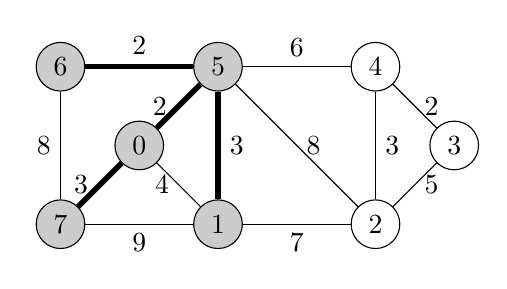
\begin{tikzpicture}
	\node[fill=black!20] (6) at (-1, 0) [circle, draw] {$6$};
	\node[fill=black!20] (5) at (1,0) [circle, draw] {$5$};
	\node (4) at (3,0) [circle, draw] {$4$};
		\node[fill=black!20] (0) at (0,-1) [circle, draw] {$0$};
		\node (3) at (4,-1) [circle, draw] {$3$};
			\node[fill=black!20] (1) at (1, -2) [circle, draw] {$1$};
			\node[fill=black!20] (7) at (-1, -2) [circle, draw] {$7$};
			\node (2) at (3, -2) [circle, draw] {$2$};
	\draw[line width=2pt][-] (0) to node [left] {2} (5);
	\draw[line width=2pt][-] (0) to node [left] {3} (7);
	\draw[-] (0) to node [left] {4} (1);
	\draw[line width=2pt][-] (1) to node [right] {3} (5);
	\draw[-] (1) to node [below] {7} (2);
	\draw[-] (1) to node [below] {9} (7);
	\draw[-] (2) to node [right] {8} (5);
	\draw[-] (2) to node [right] {3} (4);
	\draw[-] (2) to node [right] {5} (3);
	\draw[-] (3) to node [right] {2} (4);
	\draw[-] (4) to node [above] {6} (5);
	\draw[line width=2pt][-] (5) to node [above] {2} (6);
	\draw[-] (6) to node [left] {8} (7);			
	\end{tikzpicture}}
	&~& \textbf{$i$} & 				\textbf{0} & \textbf{1} & \textbf{2} & \textbf{3} & 		\textbf{4} & 		\textbf{5} & \textbf{6} & 		\textbf{7}\\
	&~& \textbf{$Nearest[i]$} & 	\textbf{2} & \textbf{0} & \textbf{7} & \textbf{$\infty$} &  \textbf{6} & 		\textbf{3} & \textbf{2} &		\textbf{3}\\
	&~& \textbf{$Parent[i]$} & 		\textbf{5} & \textbf{-1} &\textbf{1} & \textbf{-} & 		\textbf{5} & 		\textbf{1} & \textbf{5} & 		\textbf{0}\\
	&~& \textbf{$InTheTree[i]$} & 	\textbf{T} & \textbf{T} & \textbf{F} & \textbf{F} &		    \textbf{F} & 		\textbf{T} & \textbf{T} & 		\textbf{T}\\
	&~& \textbf{$Weight$}& \multicolumn{7}{l}{10} & \\
	&~& ~& \multicolumn{7}{l}{~} & \\
	&~& ~& \multicolumn{7}{l}{~} & \\
	&~& ~& \multicolumn{7}{l}{~} & \\
	\hline
\end{tabular}

\begin{tabular}{| r | r | r | r | r | r | r | r | r | r | r |}
	\multicolumn{10}{l}{Stage 6}\\
	\hline
	\multirow{4}{*}{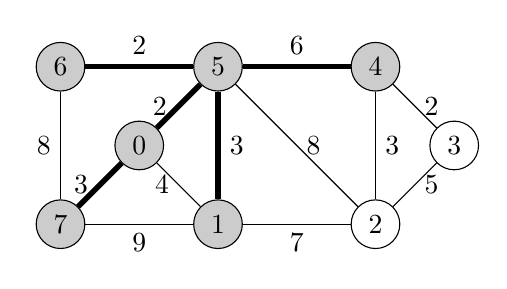
\begin{tikzpicture}
	\node[fill=black!20] (6) at (-1, 0) [circle, draw] {$6$};
	\node[fill=black!20] (5) at (1,0) [circle, draw] {$5$};
	\node[fill=black!20] (4) at (3,0) [circle, draw] {$4$};
		\node[fill=black!20] (0) at (0,-1) [circle, draw] {$0$};
		\node (3) at (4,-1) [circle, draw] {$3$};
			\node[fill=black!20] (1) at (1, -2) [circle, draw] {$1$};
			\node[fill=black!20] (7) at (-1, -2) [circle, draw] {$7$};
			\node (2) at (3, -2) [circle, draw] {$2$};
	\draw[line width=2pt][-] (0) to node [left] {2} (5);
	\draw[line width=2pt][-] (0) to node [left] {3} (7);
	\draw[-] (0) to node [left] {4} (1);
	\draw[line width=2pt][-] (1) to node [right] {3} (5);
	\draw[-] (1) to node [below] {7} (2);
	\draw[-] (1) to node [below] {9} (7);
	\draw[-] (2) to node [right] {8} (5);
	\draw[-] (2) to node [right] {3} (4);
	\draw[-] (2) to node [right] {5} (3);
	\draw[-] (3) to node [right] {2} (4);
	\draw[line width=2pt][-] (4) to node [above] {6} (5);
	\draw[line width=2pt][-] (5) to node [above] {2} (6);
	\draw[-] (6) to node [left] {8} (7);			
	\end{tikzpicture}}
	&~& \textbf{$i$} & 				\textbf{0} & \textbf{1} & \textbf{2} & \textbf{3} & 		\textbf{4} & 		\textbf{5} & \textbf{6} & 		\textbf{7}\\
	&~& \textbf{$Nearest[i]$} & 	\textbf{2} & \textbf{0} & \textbf{3} & \textbf{2} &		    \textbf{6} & 		\textbf{3} & \textbf{2} &		\textbf{3}\\
	&~& \textbf{$Parent[i]$} & 		\textbf{5} & \textbf{-1} &\textbf{4} & \textbf{4} & 		\textbf{5} & 		\textbf{1} & \textbf{5} & 		\textbf{0}\\
	&~& \textbf{$InTheTree[i]$} & 	\textbf{T} & \textbf{T} & \textbf{F} & \textbf{F} &		    \textbf{T} & 		\textbf{T} & \textbf{T} & 		\textbf{T}\\
	&~& \textbf{$Weight$}& \multicolumn{7}{l}{16} & \\
	&~& ~& \multicolumn{7}{l}{~} & \\
	&~& ~& \multicolumn{7}{l}{~} & \\
	&~& ~& \multicolumn{7}{l}{~} & \\
	\hline
\end{tabular}

\begin{tabular}{| r | r | r | r | r | r | r | r | r | r | r |}
	\multicolumn{10}{l}{Stage 7}\\
	\hline
	\multirow{4}{*}{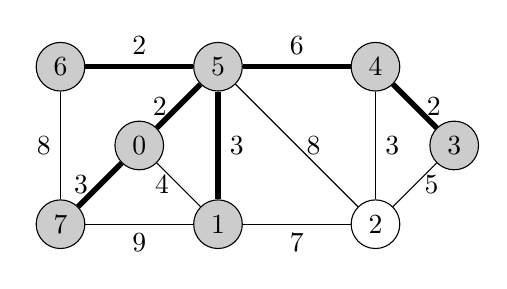
\begin{tikzpicture}
	\node[fill=black!20] (6) at (-1, 0) [circle, draw] {$6$};
	\node[fill=black!20] (5) at (1,0) [circle, draw] {$5$};
	\node[fill=black!20] (4) at (3,0) [circle, draw] {$4$};
		\node[fill=black!20] (0) at (0,-1) [circle, draw] {$0$};
		\node[fill=black!20] (3) at (4,-1) [circle, draw] {$3$};
			\node[fill=black!20] (1) at (1, -2) [circle, draw] {$1$};
			\node[fill=black!20] (7) at (-1, -2) [circle, draw] {$7$};
			\node (2) at (3, -2) [circle, draw] {$2$};
	\draw[line width=2pt][-] (0) to node [left] {2} (5);
	\draw[line width=2pt][-] (0) to node [left] {3} (7);
	\draw[-] (0) to node [left] {4} (1);
	\draw[line width=2pt][-] (1) to node [right] {3} (5);
	\draw[-] (1) to node [below] {7} (2);
	\draw[-] (1) to node [below] {9} (7);
	\draw[-] (2) to node [right] {8} (5);
	\draw[-] (2) to node [right] {3} (4);
	\draw[-] (2) to node [right] {5} (3);
	\draw[line width=2pt][-] (3) to node [right] {2} (4);
	\draw[line width=2pt][-] (4) to node [above] {6} (5);
	\draw[line width=2pt][-] (5) to node [above] {2} (6);
	\draw[-] (6) to node [left] {8} (7);			
	\end{tikzpicture}}
	&~& \textbf{$i$} & 				\textbf{0} & \textbf{1} & \textbf{2} & \textbf{3} & 		\textbf{4} & 		\textbf{5} & \textbf{6} & 		\textbf{7}\\
	&~& \textbf{$Nearest[i]$} & 	\textbf{2} & \textbf{0} & \textbf{3} & \textbf{2} &		    \textbf{6} & 		\textbf{3} & \textbf{2} &		\textbf{3}\\
	&~& \textbf{$Parent[i]$} & 		\textbf{5} & \textbf{-1} &\textbf{4} & \textbf{4} & 		\textbf{5} & 		\textbf{1} & \textbf{5} & 		\textbf{0}\\
	&~& \textbf{$InTheTree[i]$} & 	\textbf{T} & \textbf{T} & \textbf{F} & \textbf{T} &		    \textbf{T} & 		\textbf{T} & \textbf{T} & 		\textbf{T}\\
	&~& \textbf{$Weight$}& \multicolumn{7}{l}{18} & \\
	&~& ~& \multicolumn{7}{l}{~} & \\
	&~& ~& \multicolumn{7}{l}{~} & \\
	&~& ~& \multicolumn{7}{l}{~} & \\
	\hline
\end{tabular}


\begin{tabular}{| r | r | r | r | r | r | r | r | r | r | r |}
	\multicolumn{10}{l}{Final}\\
	\hline
	\multirow{4}{*}{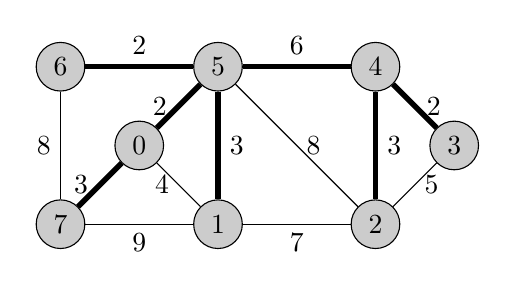
\begin{tikzpicture}
	\node[fill=black!20] (6) at (-1, 0) [circle, draw] {$6$};
	\node[fill=black!20] (5) at (1,0) [circle, draw] {$5$};
	\node[fill=black!20] (4) at (3,0) [circle, draw] {$4$};
		\node[fill=black!20] (0) at (0,-1) [circle, draw] {$0$};
		\node[fill=black!20] (3) at (4,-1) [circle, draw] {$3$};
			\node[fill=black!20] (1) at (1, -2) [circle, draw] {$1$};
			\node[fill=black!20] (7) at (-1, -2) [circle, draw] {$7$};
			\node[fill=black!20] (2) at (3, -2) [circle, draw] {$2$};
	\draw[line width=2pt][-] (0) to node [left] {2} (5);
	\draw[line width=2pt][-] (0) to node [left] {3} (7);
	\draw[-] (0) to node [left] {4} (1);
	\draw[line width=2pt][-] (1) to node [right] {3} (5);
	\draw[-] (1) to node [below] {7} (2);
	\draw[-] (1) to node [below] {9} (7);
	\draw[-] (2) to node [right] {8} (5);
	\draw[line width=2pt][-] (2) to node [right] {3} (4);
	\draw[-] (2) to node [right] {5} (3);
	\draw[line width=2pt][-] (3) to node [right] {2} (4);
	\draw[line width=2pt][-] (4) to node [above] {6} (5);
	\draw[line width=2pt][-] (5) to node [above] {2} (6);
	\draw[-] (6) to node [left] {8} (7);			
	\end{tikzpicture}}
	&~& ~& \multicolumn{7}{l}{~} & \\
	&~& ~& \multicolumn{7}{l}{~} & \\
	&~& ~& \multicolumn{7}{l}{~} & \\
	&~& ~& \multicolumn{7}{l}{~} & \\
	&~& ~& \multicolumn{7}{l}{After stage 7, array $Parent$ is now complete and implements} & \\
	&~& ~& \multicolumn{7}{l}{a minimum spanning tree with weight 21.} & \\
	&~& ~& \multicolumn{7}{l}{~} & \\
	&~& ~& \multicolumn{7}{l}{~} & \\
	\hline
\end{tabular}

\end{itemize}

\newpage
 %%%%%%%%%%%%%%%%
%	#4	-	P 393, #12.17
%%%%%%%%%%%%%%%% 
 \fbox{4} ~~ Trace the action of procedure $Dijkstra$ for the following digraph with initial vertex $r=2$.
~\\
\begin{tabular}{| r | r | r | r | r | r | r | r | r |}
	\multicolumn{8}{l}{Stage 1}\\
	\hline
	\multirow{4}{*}{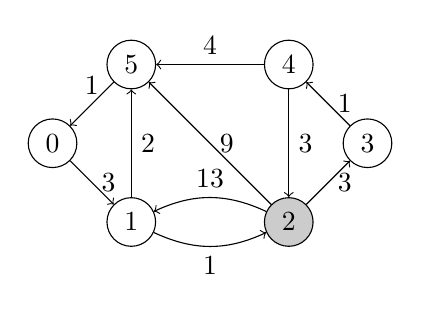
\begin{tikzpicture}
	\node (5) at (1,0) [circle, draw] {$5$};
	\node (4) at (3,0) [circle, draw] {$4$};
		\node (0) at (0,-1) [circle, draw] {$0$};
		\node (3) at (4,-1) [circle, draw] {$3$};
			\node (1) at (1, -2) [circle, draw] {$1$};
			\node[fill=black!20] (2) at (3, -2) [circle, draw] {$2$};
	\draw[->] (0) to node [right] {3} (1);		
	\draw[->] (1) to node [right] {2} (5);
	\draw[->] (1) to [bend right=25] node [below] {1} (2);
	\draw[->] (2) to node [right] {3} (3);
	\draw[->] (2) to node [right] {9} (5);
	\draw[->] (2) to [bend right=25] node [above] {13} (1);
	\draw[->] (3) to node [right] {1} (4);
	\draw[->] (4) to node [above] {4} (5);
	\draw[->] (4) to node [right] {3} (2);
	\draw[->] (5) to node [above] {1} (0);
	\end{tikzpicture}}
	&~& \textbf{$i$} & 				\textbf{0} & \textbf{1} & \textbf{2} & \textbf{3} & \textbf{4} & \textbf{5} \\
	&~& \textbf{$Dist[i]$} & 		\textbf{$\infty$} & \textbf{13} & \textbf{0} & \textbf{3} & \textbf{$\infty$} & \textbf{9} \\
	&~& \textbf{$Parent[i]$} & 		\textbf{-} & \textbf{2} & \textbf{-1} & \textbf{2} & \textbf{-} & \textbf{2} \\
	&~& \textbf{$InTheTree[i]$} & 	\textbf{F} & \textbf{F} & \textbf{T} & \textbf{F} & \textbf{F} & \textbf{F} \\
	&~& \textbf{$Total~Distance$}& \multicolumn{5}{l}{0} & \\
	&~& ~& \multicolumn{5}{l}{~} & \\
	&~& ~& \multicolumn{5}{l}{~} & \\
	&~& ~& \multicolumn{5}{l}{~} & \\
	\hline
\end{tabular}

\begin{tabular}{| r | r | r | r | r | r | r | r | r |}
	\multicolumn{8}{l}{Stage 2}\\
	\hline
	\multirow{4}{*}{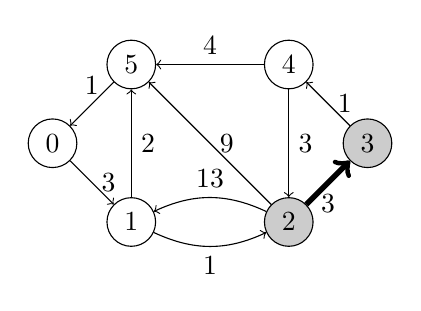
\begin{tikzpicture}
	\node (5) at (1,0) [circle, draw] {$5$};
	\node (4) at (3,0) [circle, draw] {$4$};
		\node (0) at (0,-1) [circle, draw] {$0$};
		\node[fill=black!20] (3) at (4,-1) [circle, draw] {$3$};
			\node (1) at (1, -2) [circle, draw] {$1$};
			\node[fill=black!20] (2) at (3, -2) [circle, draw] {$2$};
	\draw[->] (0) to node [right] {3} (1);		
	\draw[->] (1) to node [right] {2} (5);
	\draw[->] (1) to [bend right=25] node [below] {1} (2);
	\draw[line width=2pt][->] (2) to node [below] {3} (3);
	\draw[->] (2) to node [right] {9} (5);
	\draw[->] (2) to [bend right=25] node [above] {13} (1);
	\draw[->] (3) to node [right] {1} (4);
	\draw[->] (4) to node [above] {4} (5);
	\draw[->] (4) to node [right] {3} (2);
	\draw[->] (5) to node [above] {1} (0);
	\end{tikzpicture}}
	&~& \textbf{$i$} & 				\textbf{0} & \textbf{1} & \textbf{2} & \textbf{3} & \textbf{4} & \textbf{5} \\
	&~& \textbf{$Dist[i]$} & 		\textbf{$\infty$} & \textbf{13} & \textbf{0} & \textbf{3} & \textbf{4} & \textbf{9} \\
	&~& \textbf{$Parent[i]$} & 		\textbf{-} & \textbf{2} & \textbf{-1} & \textbf{2} & \textbf{3} & \textbf{2} \\
	&~& \textbf{$InTheTree[i]$} & 	\textbf{F} & \textbf{F} & \textbf{T} & \textbf{T} & \textbf{F} & \textbf{F} \\
	&~& \textbf{$Total~Distance$}& \multicolumn{5}{l}{3} & \\
	&~& ~& \multicolumn{5}{l}{~} & \\
	&~& ~& \multicolumn{5}{l}{~} & \\
	&~& ~& \multicolumn{5}{l}{~} & \\
	\hline
\end{tabular}

\begin{tabular}{| r | r | r | r | r | r | r | r | r |}
	\multicolumn{8}{l}{Stage 3}\\
	\hline
	\multirow{4}{*}{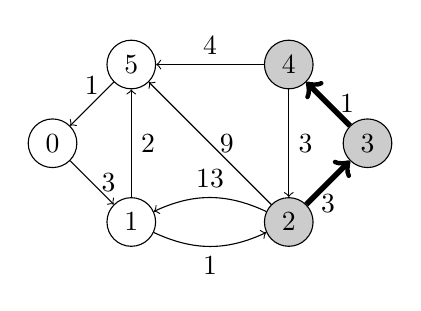
\begin{tikzpicture}
	\node (5) at (1,0) [circle, draw] {$5$};
	\node[fill=black!20] (4) at (3,0) [circle, draw] {$4$};
		\node (0) at (0,-1) [circle, draw] {$0$};
		\node[fill=black!20] (3) at (4,-1) [circle, draw] {$3$};
			\node (1) at (1, -2) [circle, draw] {$1$};
			\node[fill=black!20] (2) at (3, -2) [circle, draw] {$2$};
	\draw[->] (0) to node [right] {3} (1);		
	\draw[->] (1) to node [right] {2} (5);
	\draw[->] (1) to [bend right=25] node [below] {1} (2);
	\draw[line width=2pt][->] (2) to node [below] {3} (3);
	\draw[->] (2) to node [right] {9} (5);
	\draw[->] (2) to [bend right=25] node [above] {13} (1);
	\draw[line width=2pt][->] (3) to node [right] {1} (4);
	\draw[->] (4) to node [above] {4} (5);
	\draw[->] (4) to node [right] {3} (2);
	\draw[->] (5) to node [above] {1} (0);
	\end{tikzpicture}}
	&~& \textbf{$i$} & 				\textbf{0} & \textbf{1} & \textbf{2} & \textbf{3} & \textbf{4} & \textbf{5} \\
	&~& \textbf{$Dist[i]$} & 		\textbf{$\infty$} & \textbf{13} & \textbf{0} & \textbf{3} & \textbf{4} & \textbf{8} \\
	&~& \textbf{$Parent[i]$} & 		\textbf{-} & \textbf{2} & \textbf{-1} & \textbf{2} & \textbf{3} & \textbf{4} \\
	&~& \textbf{$InTheTree[i]$} & 	\textbf{F} & \textbf{F} & \textbf{T} & \textbf{T} & \textbf{T} & \textbf{F} \\
	&~& \textbf{$Total~Distance$}& \multicolumn{5}{l}{4} & \\
	&~& ~& \multicolumn{5}{l}{~} & \\
	&~& ~& \multicolumn{5}{l}{~} & \\
	&~& ~& \multicolumn{5}{l}{~} & \\
	\hline
\end{tabular}

\begin{tabular}{| r | r | r | r | r | r | r | r | r |}
	\multicolumn{8}{l}{Stage 4}\\
	\hline
	\multirow{4}{*}{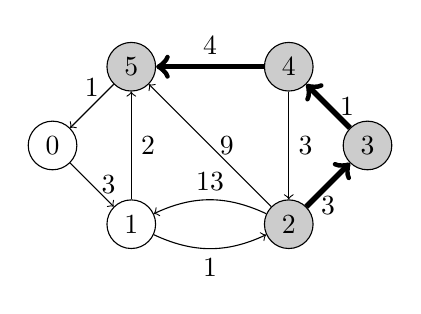
\begin{tikzpicture}
	\node[fill=black!20] (5) at (1,0) [circle, draw] {$5$};
	\node[fill=black!20] (4) at (3,0) [circle, draw] {$4$};
		\node (0) at (0,-1) [circle, draw] {$0$};
		\node[fill=black!20] (3) at (4,-1) [circle, draw] {$3$};
			\node (1) at (1, -2) [circle, draw] {$1$};
			\node[fill=black!20] (2) at (3, -2) [circle, draw] {$2$};
	\draw[->] (0) to node [right] {3} (1);		
	\draw[->] (1) to node [right] {2} (5);
	\draw[->] (1) to [bend right=25] node [below] {1} (2);
	\draw[line width=2pt][->] (2) to node [below] {3} (3);
	\draw[->] (2) to node [right] {9} (5);
	\draw[->] (2) to [bend right=25] node [above] {13} (1);
	\draw[line width=2pt][->] (3) to node [right] {1} (4);
	\draw[line width=2pt][->] (4) to node [above] {4} (5);
	\draw[->] (4) to node [right] {3} (2);
	\draw[->] (5) to node [above] {1} (0);
	\end{tikzpicture}}
	&~& \textbf{$i$} & 				\textbf{0} & \textbf{1} & \textbf{2} & \textbf{3} & \textbf{4} & \textbf{5} \\
	&~& \textbf{$Dist[i]$} & 		\textbf{9} & \textbf{13} & \textbf{0} & \textbf{3} & \textbf{4} & \textbf{8} \\
	&~& \textbf{$Parent[i]$} & 		\textbf{5} & \textbf{2} & \textbf{-1} & \textbf{2} & \textbf{3} & \textbf{4} \\
	&~& \textbf{$InTheTree[i]$} & 	\textbf{F} & \textbf{F} & \textbf{T} & \textbf{T} & \textbf{T} & \textbf{T} \\
	&~& \textbf{$Total~Distance$}& \multicolumn{5}{l}{8} & \\
	&~& ~& \multicolumn{5}{l}{~} & \\
	&~& ~& \multicolumn{5}{l}{~} & \\
	&~& ~& \multicolumn{5}{l}{~} & \\
	\hline
\end{tabular}

\begin{tabular}{| r | r | r | r | r | r | r | r | r |}
	\multicolumn{8}{l}{Stage 5}\\
	\hline
	\multirow{4}{*}{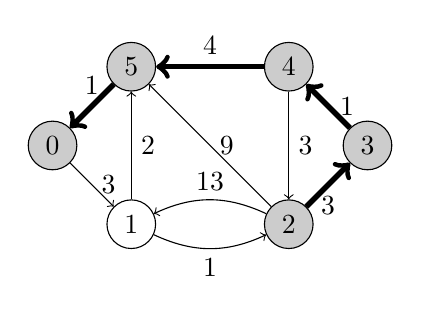
\begin{tikzpicture}
	\node[fill=black!20] (5) at (1,0) [circle, draw] {$5$};
	\node[fill=black!20] (4) at (3,0) [circle, draw] {$4$};
		\node[fill=black!20] (0) at (0,-1) [circle, draw] {$0$};
		\node[fill=black!20] (3) at (4,-1) [circle, draw] {$3$};
			\node (1) at (1, -2) [circle, draw] {$1$};
			\node[fill=black!20] (2) at (3, -2) [circle, draw] {$2$};
	\draw[->] (0) to node [right] {3} (1);		
	\draw[->] (1) to node [right] {2} (5);
	\draw[->] (1) to [bend right=25] node [below] {1} (2);
	\draw[line width=2pt][->] (2) to node [below] {3} (3);
	\draw[->] (2) to node [right] {9} (5);
	\draw[->] (2) to [bend right=25] node [above] {13} (1);
	\draw[line width=2pt][->] (3) to node [right] {1} (4);
	\draw[line width=2pt][->] (4) to node [above] {4} (5);
	\draw[->] (4) to node [right] {3} (2);
	\draw[line width=2pt][->] (5) to node [above] {1} (0);
	\end{tikzpicture}}
	&~& \textbf{$i$} & 				\textbf{0} & \textbf{1} & \textbf{2} & \textbf{3} & \textbf{4} & \textbf{5} \\
	&~& \textbf{$Dist[i]$} & 		\textbf{9} & \textbf{12} & \textbf{0} & \textbf{3} & \textbf{4} & \textbf{8} \\
	&~& \textbf{$Parent[i]$} & 		\textbf{5} & \textbf{0} & \textbf{-1} & \textbf{2} & \textbf{3} & \textbf{4} \\
	&~& \textbf{$InTheTree[i]$} & 	\textbf{T} & \textbf{F} & \textbf{T} & \textbf{T} & \textbf{T} & \textbf{T} \\
	&~& \textbf{$Total~Distance$}& \multicolumn{5}{l}{9} & \\
	&~& ~& \multicolumn{5}{l}{~} & \\
	&~& ~& \multicolumn{5}{l}{~} & \\
	&~& ~& \multicolumn{5}{l}{~} & \\
	\hline
\end{tabular}

Because Dijkstra's algorithm terminates after only $n-1$ stages, the algorithm is complete and we add $Node~1$ for a final cost/distance of 12. \\
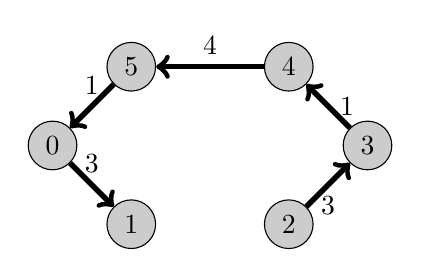
\begin{tikzpicture}
\node[fill=black!20] (5) at (1,0) [circle, draw] {$5$};
\node[fill=black!20] (4) at (3,0) [circle, draw] {$4$};
	\node[fill=black!20] (0) at (0,-1) [circle, draw] {$0$};
	\node[fill=black!20] (3) at (4,-1) [circle, draw] {$3$};
		\node[fill=black!20] (1) at (1, -2) [circle, draw] {$1$};
		\node[fill=black!20] (2) at (3, -2) [circle, draw] {$2$};
\draw[line width=2pt][->] (0) to node [above] {3} (1);		
\draw[line width=2pt][->] (2) to node [below] {3} (3);
\draw[line width=2pt][->] (3) to node [right] {1} (4);
\draw[line width=2pt][->] (4) to node [above] {4} (5);
\draw[line width=2pt][->] (5) to node [above] {1} (0);
\end{tikzpicture}


~\\


 %%%%%%%%%%%%%%%%
%	#5	-	P 233, #7.5
%%%%%%%%%%%%%%%% 
 \fbox{5} For $C=30$, we can instantly discard $i=1$ since its weight is $>30$.  Then, we'll add $i=2,3,4,6$ for $w=29$ and $v=95$.  That leaves $i=0,7$ as options, and to choose the higher value, we chose $\frac{1}{30}th$ of $i=0$ for a $v=2$.  We've met our capacity with a final value of $v=97$. \\
~\\

%%%%%%%%%%%%%%%%
%	#6	-	P 262, #8.10
%%%%%%%%%%%%%%%% 
 \fbox{6} Design and analyze an algorithm $MultInt$ for multiplying large integers.\\
~\\
The problem of dealing with arbitrarily large polynomials is similar to the problem of arbitrarily large integers.  Thus, assuming that the integers have the same number of digits, we can base our algorithm on $PolyMult1$ and instead of splitting polynomials, we will just split the integer, and instead of multiplying by $x$, we use our base-10.  Therefore, $PolyMult1$ will be transformed into $MultInt$ with integers $A=a_1+a_210^d+,B=b_1+b_210^d$ and the analysis is also the same as $PolyMult1$ with $W(n)=\Theta (n^{log_23})$\\
~\\
\textbf{function} $MultInt(A,B,n)$ \textbf{recursive}\\
\textbf{Input:} A=LargeInt, B=LargeInt, n=positive int (length of A,B)\\
\textbf{Output:} AB (product)\\
~~~ if $n=1$ then\\
~~~~~~ return(AB)\\
~~~ else\\
~~~~~~ $d \leftarrow \lceil n/2 \rceil$\\
~~~~~~ $Split(A,a_1,a_2)$\\
~~~~~~ $Split(B,b_1,b_2)$\\
~~~~~~ $C \leftarrow MultInt(a_2,b_2,d)$\\
~~~~~~ $D \leftarrow MultInt(a_1+a_2,b_1+b_2,d)$\\
~~~~~~ $E \leftarrow MultInt(a_1,b_1,d)$\\
~~~~~~ \textbf{return}$(10^{2d}C+10^d(D-C-E)+E)$\\
~~~ \textbf{end if}\\
\textbf{end} $MultInt$\\
~\\
~\\

~\\
\newpage
%%%%%%%%%%%%%%%%
%	#7	-	P 262, #8.13
%%%%%%%%%%%%%%%% 
 \fbox{7} Verify Proposition 8.4.4.
~\\
To verify this, we need the following to hold:\\
$AB=
\left[ 
	\begin{array}{cc}
		a_{00} & a_{01}\\
		a_{10} & a_{11} 
	\end{array} 
\right]
\left[ 
	\begin{array}{cc}
		b_{00} & b_{01}\\
		b_{10} & b_{11}
	\end{array} 
\right]$\\
$=
\left[ 
	\begin{array}{cc}
		a_{00}b_{00}+a_{01}b_{10} & a_{00}b_{01}+a_{01}b_{11}\\
		a_{10}b_{00}+a_{11}b_{10} & a_{10}b_{01}+a_{11}b_{11} 
	\end{array} 
\right]
=
\left[ 
	\begin{array}{cc}
		m_1+m_4-m_5+m_7 & m_3+m_5\\
		m_2+m_4 & m_1+m_3-m_2+m_6 
	\end{array} 
\right]$\\


Where $m_x$ is defined in the following:\\
$m_1=(a_{00}+a_{11})(b_{00}+b_{11})$\\
$m_2=(a_{10}+a_{11})(b_{00})$\\
$m_3=(a_{00})(b_{01}-b_{11})$\\
$m_4=(a_{11})(b_{10}-b_{00})$\\
$m_5=(a_{00}+a_{01})(b_{11})$\\
$m_6=(a_{10}-a_{00})(b_{00}+b_{01})$\\
$m_7=(a_{01}-a_{11})(b_{10}+b_{11})$\\

Thus, expanding the last matrix, we have:\\
\begin{eqnarray*}
m_1+m_4-m_5+m_7 &=& (a_{00}+a_{11})(b_{00}+b_{11}) + (a_{11})(b_{10}-b_{00}) - (a_{00}+a_{01})(b_{11})+(a_{01}-a_{11})(b_{10}+b_{11})\\
&=& a_{00}b_{00}+a_{00}b_{11}+a_{11}b_{00}+a_{11}b_{11}+a_{11}b_{10}+a_{01}b_{11}+a_{01}b_{10} \\
&~&~~~~~~~~-a_{00}b_{11}-a_{11}b_{00}-a_{11}b_{11}-a_{11}b_{10}-a_{01}b_{11} \\
&=& a_{00}b_{00}+a_{01}b_{10}
\\
~\\
m_3+m5 &=& 	(a_{00})(b_{01}-b_{11})+(a_{00}+a_{01})(b_{11})\\
&=& a_{00}b_{01}-a_{00}b_{11}+a_{00}b_{11}+a_{01}b_{11} \\
&=& a_{00}b_{01}+a_{01}b_{11} 
\\
~\\
m_2+m_4 &=& (a_{10}+a_{11})(b_{00})+(a_{11})(b_{10}-b_{00}) \\
&=& a_{01}b_{00}+a_{11}b_{00}+a_{11}b_{10}-a_{11}b_{00} \\
&=& a_{01}b_{00}+a_{11}b_{10}
\\
~\\
m_1+m_3-m_2+m_6 &=& (a_{00}+a_{11})(b_{00}+b_{11})+(a_{00})(b_{01}-b_{11})-(a_{10}+a_{11})(b_{00})+(a_{10}-a_{00})(b_{00}+b_{01})\\
&=& a_{00}b_{00}+a_{00}b_{11}+a_{11}b_{00}+a_{11}b_{11}+a_{00}b_{01}+a_{10}b_{00}+a_{10}b_{01}\\
&&-a_{00}b_{00}-a_{00}b_{11}-a_{11}b_{00}~~~~~~~~~-a_{00}b_{01}-a_{10}b_{00}\\
&=& a_{10}b_{01}+a_{11}b_{11}
\end{eqnarray*}

\newpage
%%%%%%%%%%%%%%%%
%	#8	-	P 262, #8.17
%%%%%%%%%%%%%%%% 
 \fbox{8} 
~\\ 
$M_1=(A_{00}+A_{11})(B_{00}+B_{11})=
\left[ 
	\begin{array}{cc}
		7 & 7\\
		5 & 3 
	\end{array} 
\right]
\left[ 
	\begin{array}{cc}
		5 & 2\\
		4 & 1 
	\end{array} 
\right]$\\
	$m_1=(a_{00}+a_{11})(b_{00}+b_{11})=10 \times 6=60$\\
	$m_2=(a_{10}+a_{11})(b_{00})=8 \times 5=40$\\
	$m_3=(a_{00})(b_{01}-b_{11})=7 \times 1=7$\\
	$m_4=(a_{11})(b_{10}-b_{00})=3 \times (-1)=-3$\\
	$m_5=(a_{00}+a_{01})(b_{11})=14 \times 1=14$\\
	$m_6=(a_{10}-a_{00})(b_{00}+b_{01})=(-2) \times 7=-14$\\
	$m_7=(a_{01}-a_{11})(b_{10}+b_{11})=4 \times 5=20$\\
\fbox{\bf{$M_1$}}$=
\left[ 
	\begin{array}{cc}
		m_1+m_4-m_5+m_7 & m_3+m_5\\
		m_2+m_4 & m_1+m_3-m_2+m_6 
	\end{array} 
\right]=
\left[ 
	\begin{array}{cc}
		63 & 21\\
		37 & 13 
	\end{array} 
\right]$\\
~\\



$M_2=(A_{10}+A_{11})(B_{00})=
\left[ 
	\begin{array}{cc}
		8 & 3\\
		2 & 4 
	\end{array} 
\right]
\left[ 
	\begin{array}{cc}
		0 & 2\\
		0 & 1 
	\end{array} 
\right]$\\
	$m_1=(a_{00}+a_{11})(b_{00}+b_{11})=12$\\
	$m_2=(a_{10}+a_{11})(b_{00})=0$\\
	$m_3=(a_{00})(b_{01}-b_{11})=8$\\
	$m_4=(a_{11})(b_{10}-b_{00})=0$\\
	$m_5=(a_{00}+a_{01})(b_{11})=11$\\
	$m_6=(a_{10}-a_{00})(b_{00}+b_{01})=-12$\\
	$m_7=(a_{01}-a_{11})(b_{10}+b_{11})=1$\\
\fbox{\bf{$M_2$}}$=
\left[ 
	\begin{array}{cc}
		m_1+m_4-m_5+m_7 & m_3+m_5\\
		m_2+m_4 & m_1+m_3-m_2+m_6 
	\end{array} 
\right]	=
	\left[ 
		\begin{array}{cc}
			0 & 19\\
			0 & 8 
		\end{array} 
	\right]$\\
~\\

$M_3=(A_{00})(B_{01}-B_{11})=
\left[ 
	\begin{array}{cc}
		2 & 0\\
		3 & 0 
	\end{array} 
\right]
\left[ 
	\begin{array}{cc}
		-4 & 1\\
		-4 & -1 
	\end{array} 
\right]$\\
	$m_1=(a_{00}+a_{11})(b_{00}+b_{11})=-10$\\
	$m_2=(a_{10}+a_{11})(b_{00})=-12$\\
	$m_3=(a_{00})(b_{01}-b_{11})=4$\\
	$m_4=(a_{11})(b_{10}-b_{00})=0$\\
	$m_5=(a_{00}+a_{01})(b_{11})=-2$\\
	$m_6=(a_{10}-a_{00})(b_{00}+b_{01})=-3$\\
	$m_7=(a_{01}-a_{11})(b_{10}+b_{11})=0$\\
\fbox{\bf{$M_3$}}$=
\left[ 
	\begin{array}{cc}
		m_1+m_4-m_5+m_7 & m_3+m_5\\
		m_2+m_4 & m_1+m_3-m_2+m_6 
	\end{array} 
\right]	=
	\left[ 
		\begin{array}{cc}
			-8 & 2\\
			-12 & 3 
		\end{array} 
	\right]$\\
~\\

$M_4=(A_{11})(B_{10}-B_{00})=
\left[ 
	\begin{array}{cc}
		5 & 7\\
		2 & 3 
	\end{array} 
\right]
\left[ 
	\begin{array}{cc}
		3 & -2\\
		6 & 0 
	\end{array} 
\right]$\\
	$m_1=(a_{00}+a_{11})(b_{00}+b_{11})=24$\\
	$m_2=(a_{10}+a_{11})(b_{00})=15$\\
	$m_3=(a_{00})(b_{01}-b_{11})=-10$\\
	$m_4=(a_{11})(b_{10}-b_{00})=9$\\
	$m_5=(a_{00}+a_{01})(b_{11})=0$\\
	$m_6=(a_{10}-a_{00})(b_{00}+b_{01})=-3$\\
	$m_7=(a_{01}-a_{11})(b_{10}+b_{11})=24$\\
\fbox{\bf{$M_4$}}$=
\left[ 
	\begin{array}{cc}
		m_1+m_4-m_5+m_7 & m_3+m_5\\
		m_2+m_4 & m_1+m_3-m_2+m_6 
	\end{array} 
\right]	=
	\left[ 
		\begin{array}{cc}
			57 & -10\\
			24 & -4 
		\end{array} 
	\right]$\\
~\\

$M_5=(A_{00}+A_{01})(B_{11})=
\left[ 
	\begin{array}{cc}
		3 & 1\\
		3 & 4 
	\end{array} 
\right]
\left[ 
	\begin{array}{cc}
		5 & 0\\
		4 & 0 
	\end{array} 
\right]$\\
	$m_1=(a_{00}+a_{11})(b_{00}+b_{11})=35$\\
	$m_2=(a_{10}+a_{11})(b_{00})=35$\\
	$m_3=(a_{00})(b_{01}-b_{11})=0$\\
	$m_4=(a_{11})(b_{10}-b_{00})=-4$\\
	$m_5=(a_{00}+a_{01})(b_{11})=0$\\
	$m_6=(a_{10}-a_{00})(b_{00}+b_{01})=0$\\
	$m_7=(a_{01}-a_{11})(b_{10}+b_{11})=-12$\\
\fbox{\bf{$M_5$}}$=
\left[ 
	\begin{array}{cc}
		m_1+m_4-m_5+m_7 & m_3+m_5\\
		m_2+m_4 & m_1+m_3-m_2+m_6 
	\end{array} 
\right]	=
	\left[ 
		\begin{array}{cc}
			19 & 0\\
			31 & 0 
		\end{array} 
	\right]$\\
~\\

$M_6=(A_{10}-A_{00})(B_{00}+B_{01})=
\left[ 
	\begin{array}{cc}
		1 & -4\\
		-3 & 1 
	\end{array} 
\right]
\left[ 
	\begin{array}{cc}
		1 & 3\\
		0 & 0 
	\end{array} 
\right]$\\
	$m_1=(a_{00}+a_{11})(b_{00}+b_{11})=2$\\
	$m_2=(a_{10}+a_{11})(b_{00})=-2$\\
	$m_3=(a_{00})(b_{01}-b_{11})=3$\\
	$m_4=(a_{11})(b_{10}-b_{00})=-1$\\
	$m_5=(a_{00}+a_{01})(b_{11})=0$\\
	$m_6=(a_{10}-a_{00})(b_{00}+b_{01})=-16$\\
	$m_7=(a_{01}-a_{11})(b_{10}+b_{11})=0$\\
\fbox{\bf{$M_6$}}$=
\left[ 
	\begin{array}{cc}
		m_1+m_4-m_5+m_7 & m_3+m_5\\
		m_2+m_4 & m_1+m_3-m_2+m_6 
	\end{array} 
\right]	=
	\left[ 
		\begin{array}{cc}
			1 & 3\\
			-3 & -9 
		\end{array} 
	\right]$\\
~\\

$M_7=(A_{01}-A_{11})(B_{10}+B_{11})=
\left[ 
	\begin{array}{cc}
		-4 & -6\\
		-2 & 1 
	\end{array} 
\right]
\left[ 
	\begin{array}{cc}
		8 & 0\\
		10 & 1 
	\end{array} 
\right]$\\
	$m_1=(a_{00}+a_{11})(b_{00}+b_{11})=-27$\\
	$m_2=(a_{10}+a_{11})(b_{00})=-8$\\
	$m_3=(a_{00})(b_{01}-b_{11})=4$\\
	$m_4=(a_{11})(b_{10}-b_{00})=2$\\
	$m_5=(a_{00}+a_{01})(b_{11})=-10$\\
	$m_6=(a_{10}-a_{00})(b_{00}+b_{01})=16$\\
	$m_7=(a_{01}-a_{11})(b_{10}+b_{11})=77$\\
\fbox{\bf{$M_7$}}$=
\left[ 
	\begin{array}{cc}
		m_1+m_4-m_5+m_7 & m_3+m_5\\
		m_2+m_4 & m_1+m_3-m_2+m_6 
	\end{array} 
\right]	=
	\left[ 
		\begin{array}{cc}
			-92 & -6\\
			-6 & 1 
		\end{array} 
	\right]$\\
~\\
$AB=
	\left[ 
		\begin{array}{cc}
			M_1+M_4- M_5+M_7 & M_3+M_5\\
			M_2+M_4 & M_1+M_3-M_2+M_6 
		\end{array} 
	\right]$ 
~\\
$=
\left[ 
	\begin{array}{cccc}
		(63+57-19-92) & (21-10-6) & (-8+19) & (2+0)\\
		(37+24-31-6) & (13-4+1) & (-12+31) & (3+0)\\
		(0+57) & (19-10) & (63-8+0+1) & (21+2-19+3)\\
		(0+24) & (8-4) & (37-12-0-3) & (13+3-8-9) 
	\end{array} 
\right]
$
~\\
$=
\left[ 
	\begin{array}{cccc}
		9 & 5 & 11 & 2\\
		24 & 10 & 19 & 3\\
		57 & 9 & 56 & 7\\
		24 & 4 & 22 & -1 
	\end{array} 
\right]$

\end{flushleft}
\end{document}